\section{Teraquop volume}\label{sec:teraquop_volume}

Before we start looking at particular DCCCs in detail, we first introduce the key 
metric we use to evaluate performance throughout this work.
It is the natural generalisation of the \emph{teraquop footprint} \cite{gidney2021fault} from a `space only' picture to a `full spacetime' picture.
We call it the \emph{teraquop volume}.

\begin{definition}
    Consider a family of circuits implementing a quantum error correcting protocol, whose $j$-th member is defined on a number of qubits $n_j$ and runs for an amount of time $T_j$.
    Given a noise model and a decoder,
    the \textbf{teraquop volume} is the smallest volume $n_j T_j$ such that the probability of any spacelike and timelike logical error in the $j$-th circuit is $10^{-12}$.
\end{definition}

Here we deliberately do not specify what exactly a quantum error correcting protocol is and what it means for a set of circuits implementing one to form a family.
For a given circuit, noise model and decoder, the \emph{overall logical error rate} is the probability of any logical error -- whether spacelike or timelike -- occurring after the decoder has been applied.
In practice, an approximation of this value will be found numerically.
If there is no $(n_j, T_j)$ such that the overall logical error rate is less than $10^{-12}$, then we say the teraquop volume is infinite.
For a given code family, noise model, and physical error rate, the teraquop volume typically corresponds to a unique point $(n_j, T_j)$ rather than a smooth curve of equivalent space-time trade-offs.
That is, one cannot generally reduce the number of qubits and compensate by increasing the number of rounds (or vice versa) while maintaining the target logical error rate.

The teraquop volume is the appropriate metric for evaluating quantum error correction performance in lattice surgery computations because it accounts for space-time tradeoffs.
In surface code architectures, circuit depth can be reduced at the cost of increased qubit overhead, or vice versa \cite{lee2021even}.
A volume-based metric captures this interchangeability, making it possible to compare codes with different spatial and temporal resource requirements on equal footing.
If the teraquop footprint were used instead, codes with high qubit overhead but low circuit depth would be unfairly penalized, and vice versa.

In the next subsection we explain how we determine the teraquop volume of a DCCC.
\Cref{fig:teraquop_volume_summary} summarizes the concept of teraquop volume and the methodology used for its determination.

\subsection{Estimating the teraquop volume}\label{subsec:estimating-teraquop-volume}

\begin{figure}[p]
  \centering
    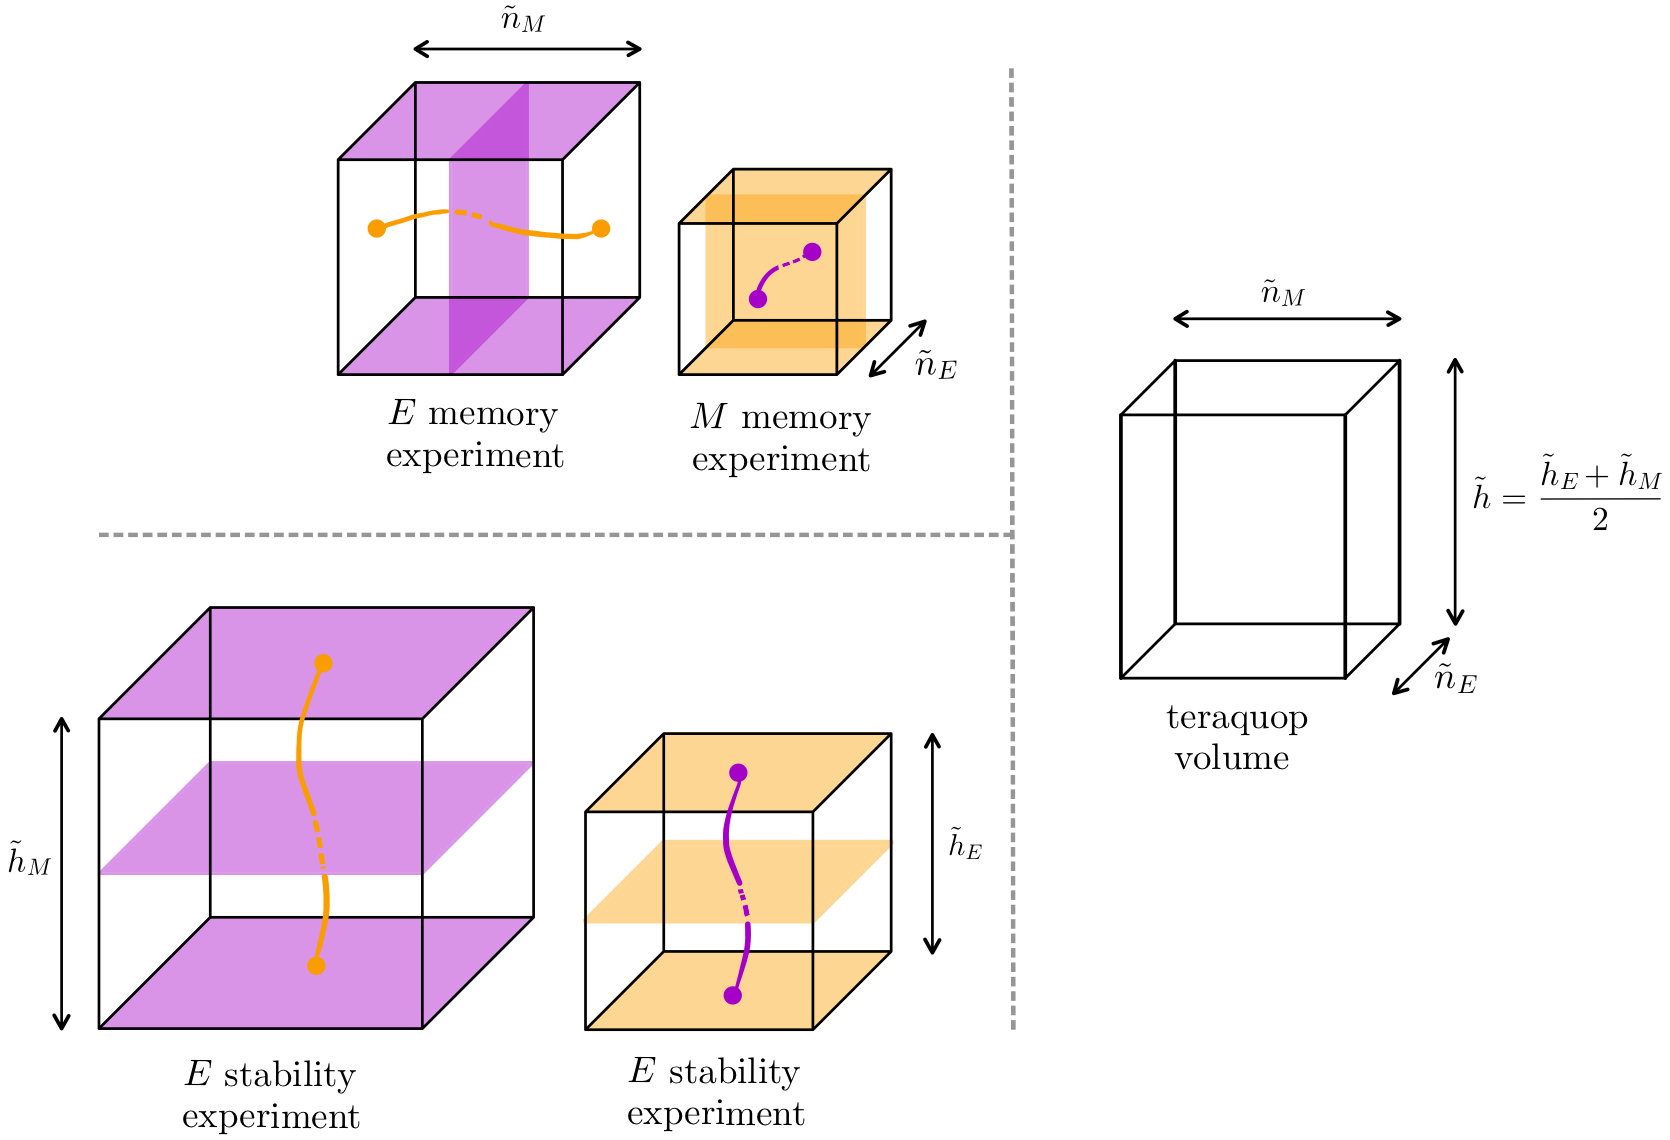
\includegraphics[width=0.9\linewidth]{figures/teraquop_volume/teraquop_volume_schematic}
    \caption{
        Schematic explaining how the teraquop volume of a DCCC is estimated.
        We perform $E$-memory experiments to estimate the number of columns $\tilde{n}_M$ of hexagons in any DCCC that reaches the teraquop regime. Then $M$-memory experiments estimate the number of rows $\tilde{n}_E$ required, and $E$- and $M$-stability experiments estimate the number of measurement rounds $\tilde{h}$ required.}
    \label{fig:teraquop_volume_summary}

    \vspace{10pt}
  
  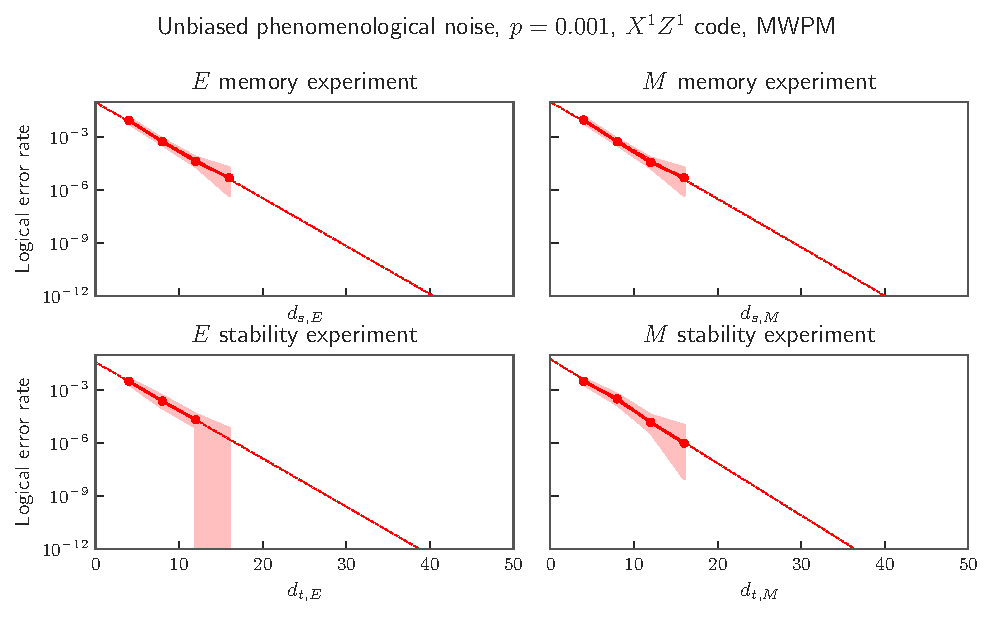
\includegraphics[width=0.9\linewidth]{figures/teraquop_volume/X1Y1Z1_X1Z1_teraquop_linefits}
    \caption{
        Plots showing line-fits to determine the minimal value of $n_E$, $n_M$  $h_E,$ and $h_M$ such that the probability of any logical error occurring is $10^{-12}$.
        The value of the $x$-axis wherever a dotted line would first cross the line $y = 10^{-12}$ is the value used for the corresponding teraquop dimension.
        The highlighted regions are computed with Sinter and show hypothesis probabilities within 1000× of the max likelihood hypothesis \cite{AG47_2024}.}
    \label{fig:X1Y1Z1_X1Z1_teraquop_linefits}
\end{figure}


\begin{figure}[t]
    \centering
    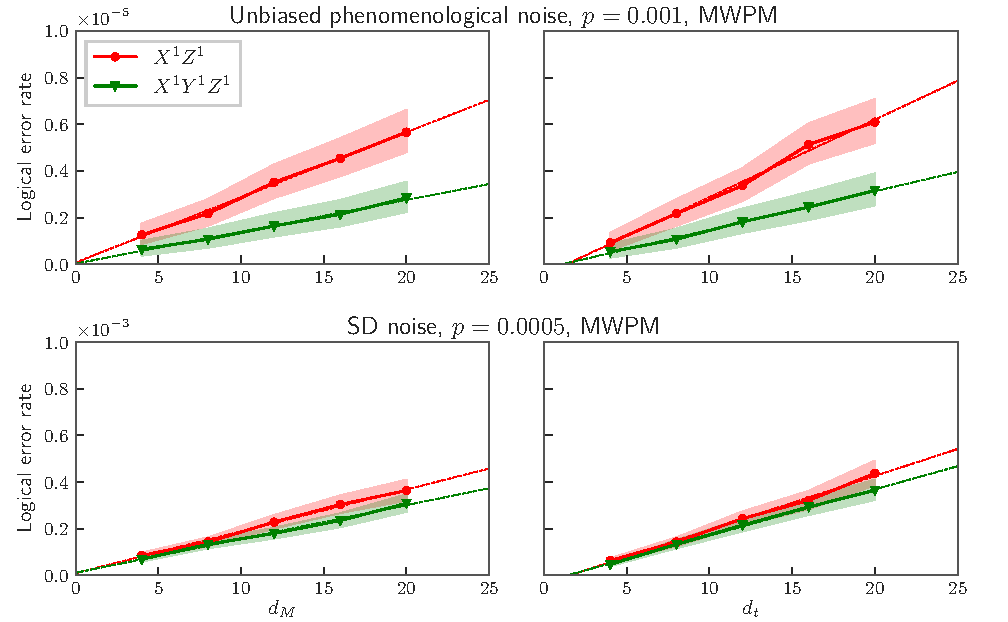
\includegraphics[width=\linewidth]{figures/teraquop_volume/volume_verification}
    \caption{
        Plots showing the logical error rate of $E$ memory experiments with varying $n_M$ and $h$. Decoding is performed with MWPM.
        The plots confirm that the probability of a spacelike logical $E$ error occurring depends linearly on $n_M$ and $h$.
        The highlighted regions are computed with Sinter and show hypothesis probabilities within 1000× of the max likelihood hypothesis \cite{AG47_2024}.
    }
    \label{fig:volume_verification}
\end{figure}

Let $n_M$ and $n_E$ denote (respectively) the number of rows and columns of hexagons in a DCCC.
For example, in \Cref{fig:edge_and_face_operator,fig:logicals_XYZ_and_XZ} we showed DCCCs with $n_M = 3$ (admittedly quite wonky) rows of hexagons, and $n_E = 4$ columns.
The value of $n_M$ determines the spacelike $M$ distance $d_{s,M}$ -- namely $d_{s,M} = \frac{4}{3}n_M$.
Similarly $n_E$ determines the spacelike $E$ distance as $d_{s,E} = n_E$.

The total number of data qubits (i.e., vertices) in a DCCC with shape $(n_M, n_E)$ is $2 n_M n_E$.
The total number of auxiliary qubits varies depending on the circuits used to perform the measurements defining the code.
For example, on a heavy-hex lattice where an auxiliary qubit is placed on each edge and measurements are performed via controlled gates and single-qubit measurements, the number of auxiliary qubits is $3 n_M n_E$, for a total of $5 n_M n_E$ qubits.
If measurements are performed via two-qubit measurements directly, then no auxiliary qubits are needed, so the total number of qubits is just $2 n_M n_E$.
For a given family of circuits, we denote the total number of qubits (the \textit{footprint}) by $f(n_M n_E)$.

Given such a family, suppose we perform $h$ rounds of measurements.
In contrast to $n_M$ and $n_E$, the value of $h$ simultaneously determines both the timelike $M$ distance and the timelike $E$ distance, denoted $d_{t,M}$ and $d_{t,E}$ respectively.
Furthermore, these timelike distances depend on the specific choice of DCCC, as we will see shortly in \Cref{sec:choosing-a-schedule}.
We say the total \textit{volume} of this circuit is $f(n_M n_E) h$.
Determining the teraquop volume requires finding the minimal value of $f(n_M n_E) h$ such that the probability of any logical error occurring is $10^{-12}$.
Although this suggests a large search space, the minimal values of $n_E$, $n_M$, and $h$ can be evaluated independently to obtain a good approximation.
This is because the probability of each type of logical error occurring (spacelike $E$ or $M$, or timelike $E$ or $M$) depends exponentially on one of $n_E$, $n_M$, and $h$, and linearly on the other two.
For example, the probability of a spacelike logical $E$ error occurring depends exponentially on $n_E$ and linearly on $n_M$ and $h$.
When the minimum value of all three independently-determined dimensions are used together, each type of logical error remains well-suppressed because the exponential dependence dominates the linear scaling.
The overall logical error rate approximates $10^{-12}$, though it may be somewhat below or above this threshold by a small constant factor.

Plots verifying this linear dependence are shown in \Cref{fig:volume_verification}.
It could be the case that for different codes the probability of each type of logical error occurring depends exponentially on one parameter and non-linearly on the other two, but we have not observed this in any of the DCCCs we have studied.
If this were to occur, we expect that the approximation method we use would still give a reasonable estimate of the teraquop volume.
To verify if our approximation method is accurate, one can simulate the overall logical error rate for the estimated minimal values of $n_E$, $n_M$, and $h$ and check if it is indeed below $10^{-12}$.

To actually find these minimal values of $n_E$, $n_M$, and $h$, we perform memory and stability experiments~\cite{gidney2022stability}.
A memory experiment means initialising a logical qubit in an eigenstate of a certain logical operator,
performing the logical identity gate for some amount of time,
then measuring this logical operator.
In the absence of noise, this measurement outcome will be deterministic, but the occurrence of certain logical errors can cause the decoder to fail and return the wrong measurement outcome.
The frequency with which these failures occur is the logical error rate for this experiment.
A stability experiment instead benchmarks how reliably the product of a large region of stabilizers can be measured~\cite{gidney2022stability}.
This tests a part of a lattice surgery operation (where the product of stabilizers measured corresponds to a logical Pauli product), or a part of an operation to move a logical operator (where the region of stabilizers is multiplied into the logical operator to move it).
Whereas a memory experiment benchmarks how well a logical observable is preserved through time, a stability experiment tests how well it is preserved through space.
Both experiments test important building blocks of a lattice surgery quantum computer.

For example, in a DCCC, an $E$ memory experiment is one in which our logical qubit is initialised in the $+1$ eigenstate of the $E$ logical operator.
Its failure rate tells us how often spacelike $M$ logical errors occur,
and depends exponentially on $n_M$ but only linearly on $n_E$ and $h$.
So for variable $d$, we can perform $E$ memory experiments with $n_M$, $n_E$ and $h$ chosen such that both spacelike distances are $d$ (i.e., $d_{s,E}(n_E) = d$ and $d_{s,M}(n_M) = d$) and both timelike distances are at least $d$ (i.e., $d_{t,E}(h) \geq d$ and $d_{t,M}(h) \geq d$).
For each $d$ we obtain a logical error rate.
The minimum $n_M(d)$ at which this logical error rate goes under $10^{-12}$ is the value of $n_M$ we will use in our teraquop volume estimation.
We fit a line to the natural log of the logical error rate versus $d$ and extrapolate this line to find the required $n_M(d)$. 
\Cref{fig:X1Y1Z1_X1Z1_teraquop_linefits} contains examples of plots showing the described line fits.

We repeat the entire procedure with the roles of $E$ and $M$ swapped to find the value of $n_E$ to use in our teraquop volume estimation.
To find the value of $h$ we use, we do essentially the same thing but with stability experiments.
An $E$ stability experiment tests for protection against timelike $M$ errors, and vice versa for an $M$ stability experiment.
Plotting the logical error rates and extrapolating gives us an estimate for the numbers of rounds of measurements $h_E$ and $h_M$ needed to ensure timelike logical $E$ and $M$ errors occur with probability less than $10^{-12}$.
We then just choose the value $h$ that we use in our teraquop volume estimation to be the mean $(h_E + h_M)/2$.
By doing this we assume that places where timelike logical $E$ and $M$ errors can occur are roughly equally prevalent in a lattice surgery computation.
Additionally, we assume that logical qubits do not need to be synchronized, meaning that lattice surgery measurements in which timelike logical $E$ errors can occur can have a different duration to ones in which timelike logical $M$ errors can occur.

\subsection{Blocks}\label{teraquop-blocks}

In the rest of this work we describe a DCCC with $n_M$ rows and $n_E$ columns of hexagons implemented for $h$ rounds of measurements as an \textit{$(n_M, n_E, h)$-block} of this DCCC.
We say it has \textit{block height} $h$, \textit{block width} $n_E$ and \textit{block depth} $n_M$.
Then we'll write $\tilde{n}_M$, $\tilde{n}_E$, $\tilde{h}_M$, and $\tilde{h}_E$ for the minimum values of $n_M$, $n_E$, $h_M$, and $h_E$ such that the corresponding logical error rates are below $10^{-12}$.
An $(\tilde{n}_M, \tilde{n}_E, \tilde{h})$-block will be referred to as a \textit{teraquop block},
with \textit{teraquop height} $\tilde{h} = (\tilde{h}_E + \tilde{h}_M)/2$, and so on.

\subsection{Limitations}\label{subsec:teraquop-limitations}

The teraquop volume is a measure of the spacetime cost of the basic unit of a lattice surgery quantum computer. As with all single-number metrics, it has its drawbacks. 
One drawback is that equal cost is attributed to space and time. 
For example, we might have two (spacetime) blocks of code with equal volume but different dimensions -- one tall and narrow, one short and wide.
In a setting where qubits are limited but time is plentiful, the tall and narrow block would be the better choice.
In contrast, if qubits are plentiful but time is limited, the short and wide block should be chosen. 
This important difference between the two blocks disappears when just looking at the teraquop volumes.

A second drawback is that the teraquop volume measure does not account for optimizations achieved by altering the measurement schedule and patch size during a computation.
Consider a circuit component in which logical qubits idle for a long time. In this scenario, there are no timelike errors to worry about.
Therefore, the logical qubits should be encoded in a circuit with low teraquop \emph{footprint}, and not necessarily low teraquop \emph{volume}.
